\section{Analysis strategy}\label{chap6:AnalysisStrategy}

The analysis strategy for the first results on the high mass search in the $\mathrm{W^+W^-}\to2\ell2\nu$ decay channel closely follows the strategy presented in the 13\TeV SM Higgs search in the $\mathrm{H}\to\mathrm{W^+W^-}\to2\ell2\nu$ channel regarding the 0 and 1 jet categories. In addition a dedicated category to the VBF production mechanism is added, given that this production mode is particularly important in the high mass region. Indeed, assuming a SM Higgs boson, the ratio of cross sections $\sigma_\mathrm{VBF}/\sigma_\mathrm{ggH}$\footnote{The ggH notation is used for the gluon-gluon fusion production mode, even in the cases where a non-SM Higgs boson is created in the process.} increases with the Higgs boson mass, making the VBF production mechanism more and more important as the mass of the resonance approaches to high values.

This analysis is affected essentially by the same background processes as the SM Higgs boson search, with the difference that in this case the SM Higgs boson processes, including all production modes, are treated as backgrounds.

In addition to requiring the events to pass the single or double lepton triggers, exactly one electron and one muon are required to be reconstructed in the event with opposite charges and a 
minimum \pt of 20\GeV for both the muon and electron. Both leptons are
required to be well identified and isolated to reject fake leptons and leptons
coming from decays in flight. To suppress background processes with three or more leptons in the final state, such as diboson or triboson production, events with any additional identified and isolated 
lepton with $\pt>10$\GeV are rejected. To suppress the contribution of the SM production of the Higgs boson at 125\GeV, \mll is requested to be higher than 50\GeV. The other event requirements are identical to the 125\GeV Higgs boson search and are described in Sec.~\ref{chap5:eventSel}.

In addition to the 0 and 1 jet categories, a specific category sensitive to the VBF production mode is defined exploiting the characteristic signature of this process, where two energetic jets are emitted in the forward region of the detector and with large $\Delta\eta$ gap. Events belonging to the VBF-enriched category are selected by requiring at least two jets with $\pt>30$\GeV, an invariant mass $m_\mathrm{jj}>500$\GeV and a gap in pseudorapidity $\Delta\eta_\mathrm{jj}>3.5$.

In addition to the transverse mass variable \mt, which is used in the analysis selection to define the DY background control region, an additional variable is defined, that from now on will be labelled as ``improved transverse mass'' \mti. This variable is defined as the invariant mass of the four momentum resulting from the sum of the two leptons four momenta ($p_{\ell\ell},\vec{p}_{\ell\ell}$)
and four momentum $\mathbf{\MET} = (\MET, \ptmiss)$, i.e.:

\begin{equation} 
\mti = \sqrt{(p_{\ell\ell}+\MET)^2-(\vec{p}_{\ell\ell}+\ptmiss)^2} \quad .
\end{equation}

This variable allows having a better sensitivity to different resonance mass hypothesis as shown in Fig.~\ref{fig:mti}, where the shape of the \mti variable is shown for different SM Higgs mass hypothesis and it is compared to the standard \mt variable. The usage of this variable also provide a good discriminating power between signal and background, which depends on the particular signal mass hypothesis.

\begin{figure}[htbp]
\centering
\subfigure{
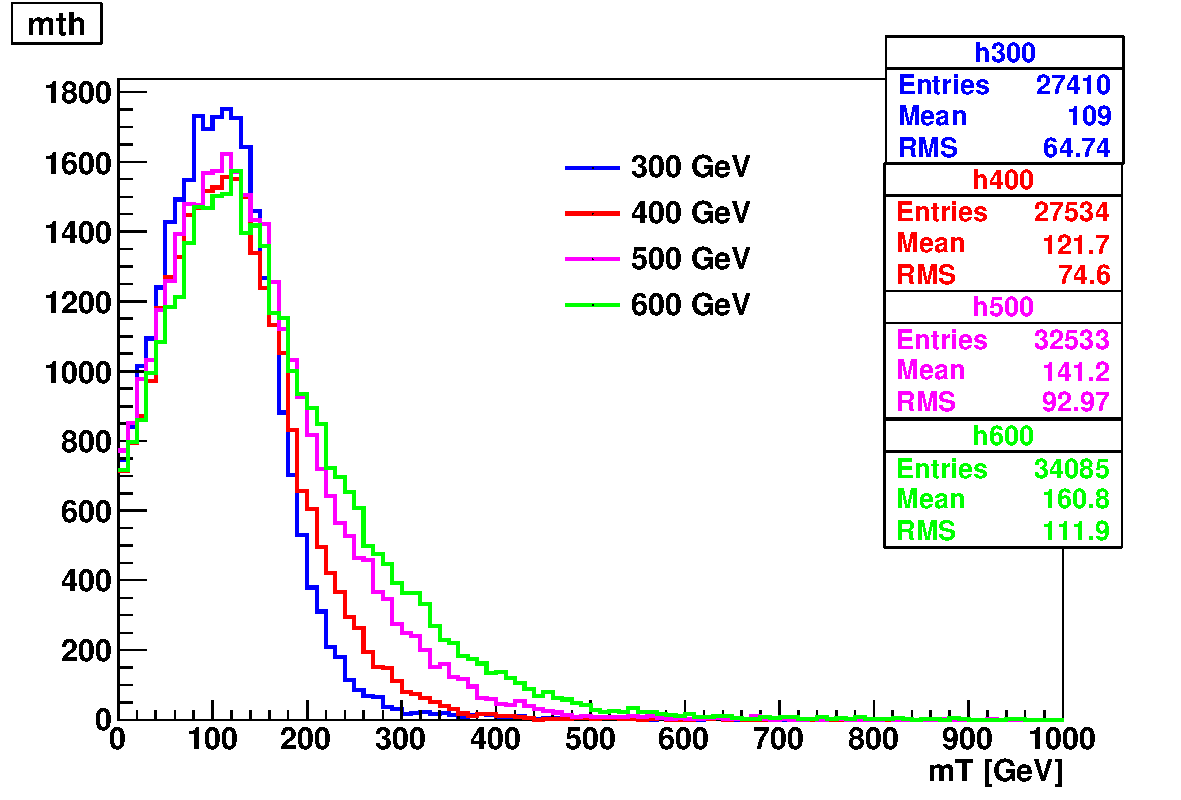
\includegraphics[width=0.45\textwidth]{images/13TeV/mT.pdf}
}
\subfigure{
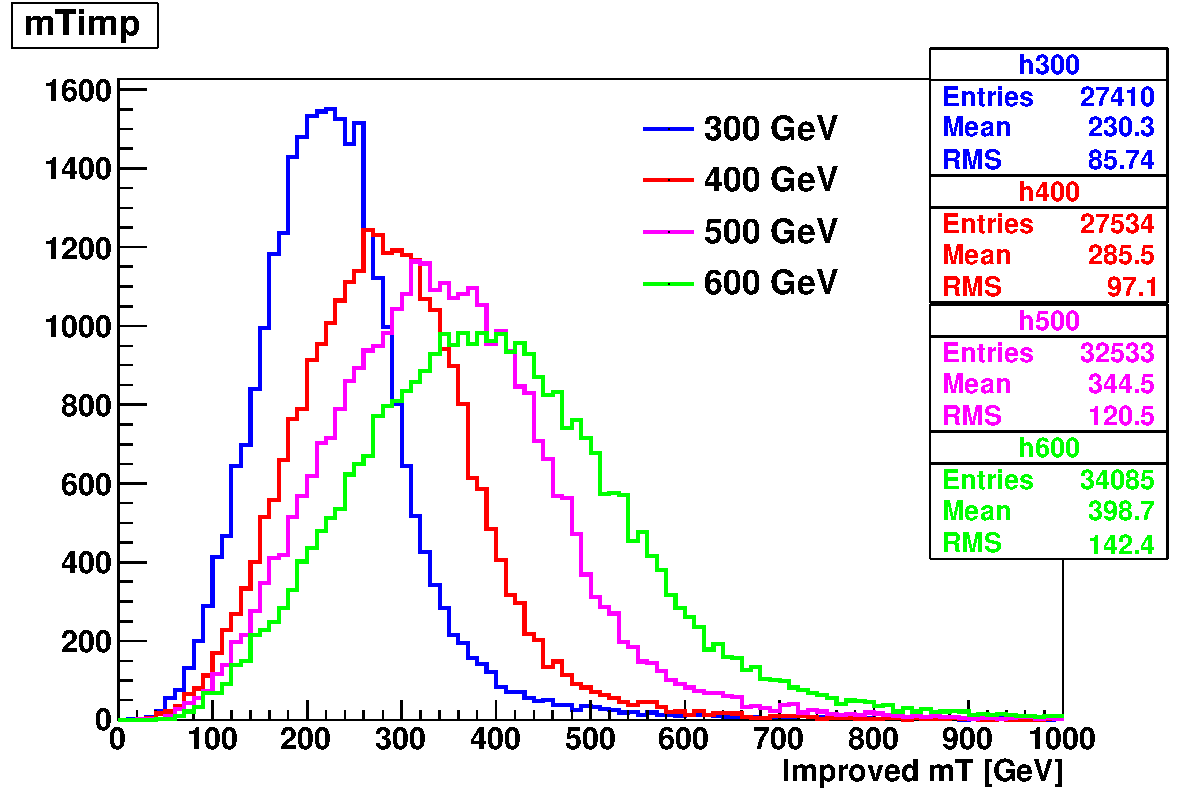
\includegraphics[width=0.45\textwidth]{images/13TeV/mTi.pdf}
}
\caption{
    Distribution of the \mt and \mti variables at generator level for different resonance mass hypothesis.}
    \label{fig:mti}
\end{figure}

The signal extraction is based on a binned maximum likelihood fit using the \mti distribution for signal and background contributions as templates. The \mti template is defined using the following bin boundaries:
\begin{itemize}
\item {\bf 0/1 jet: } [100,150,200,250,300,350,400,450,500,600,700,1000] ,
\item {\bf VBF: } [100,150,200,250,300,350,400,500,700,1000] ,
\end{itemize}
where the first number represents the lower edge of the first bin while the other numbers represent the upper edges. The last bin is an overflow bin.

In order to test different resonance decay widths hypotheses, the signal samples, which are generated with a decay width corresponding to the expected value for a SM Higgs boson at that mass ($\Gamma_\mathrm{SM}$), are reweighted to obtain the desired width value ($\Gamma'$). In particular the following values are used: $\Gamma' = \Gamma_\mathrm{SM}$, $\Gamma' = 0.49 \times \Gamma_\mathrm{SM}$, $\Gamma' = 0.25 \times \Gamma_\mathrm{SM}$ and $\Gamma' = 0.09 \times \Gamma_\mathrm{SM}$.




